\documentclass[11pt]{article}
\title{Midterm 2}
%% Language and font encodings
\usepackage[english]{babel}
\usepackage[utf8x]{inputenc}
\usepackage[T1]{fontenc}

\usepackage{helvet}

%% Sets page size and margins
\usepackage[letterpaper,top=3cm,bottom=2cm,left=3cm,right=3cm,marginparwidth=1.75cm]{geometry}

%% Useful packages
\usepackage{amsmath}
\usepackage{graphicx}
\usepackage{tcolorbox}
\usepackage{amssymb}
\usepackage{amsthm}
\usepackage{lastpage}
\usepackage{accents}
\usepackage{multicol}

% For better list numbering
\usepackage[shortlabels]{enumitem}

% Font
% \usepackage{tgbonum}


% Tikz
\usepackage{tikz}

\usetikzlibrary{calc,fit,shapes.misc,backgrounds}
\usepackage{pgfplots}
\pgfplotsset{compat = newest}
\usetikzlibrary{positioning, arrows.meta}
\usepgfplotslibrary{fillbetween}

% Headers
\usepackage{fancyhdr}
\pagestyle{fancy}

% Store \@title as \thetitle
\makeatletter
\let\thetitle\@title
\makeatother

\fancyhf{}
\lhead{\fontfamily{qbk}\fontsize{10}{11}\selectfont ECON 3535}
\rhead{\fontfamily{qbk}\fontsize{10}{11}\selectfont \thetitle}
\rfoot{\fontfamily{qbk}\fontsize{10}{11}\selectfont \thepage}


% Sections and Subsections

% define colors
\definecolor{buff-gold}{HTML}{CFB87C}
\definecolor{buff-grey}{HTML}{565A5C}
% custom tcolorbox
\tcbset{colframe=buff-gold, colback=white!100!black}

% new page per section
\usepackage{titlesec}
\newcommand{\sectionbreak}{\clearpage}
% change style of section
\usepackage{sectsty}
\sectionfont{\color{buff-gold} \fontfamily{qbk}\selectfont}
\subsectionfont{\color{buff-grey} \fontfamily{qbk}\selectfont}
\subsubsectionfont{\color{buff-grey} \fontfamily{qbk}\selectfont}



\newtoggle{INCLUDEANSWERS}
\togglefalse{INCLUDEANSWERS}

\newcommand{\answer}[1]{\iftoggle{INCLUDEANSWERS}{{\color{violet!70!white}\textbf{Solution:} #1}}{}}

\newtoggle{INCLUDEPOINTS}
\toggletrue{INCLUDEPOINTS}
\newcommand{\points}[1]{\iftoggle{INCLUDEPOINTS}{{\color{blue!70!white}(#1 pts.)}}{}}


\begin{document}
\emph{Good luck to you!}

% \vspace*{5mm}
\textbf{Multiple Choice}

\begin{enumerate}
  \item \points{5} Why are local pollutants much easier to regulate than global pollutants?

  \begin{enumerate}
    \item Global pollutants have no immediate impact on human health, while local pollutants do.
    \item A locality faces all the benefits of reducing a local pollutant, but does not face all the benefits of reducing a global pollutant.
    \item Local pollutants are produced in larger quantities and are more difficult to track.
    \item Global pollutants are more visible and, therefore, receive more public attention and regulatory scrutiny.  
  \end{enumerate}

  \answer{(b)}

  \item \points{5} Which of the following is an example of the rebound effect?
  \begin{enumerate}
    \item A company invests in energy-efficient lighting and reduces its overall electricity consumption by 20\%.
    \item A homeowner installs solar panels and sells excess electricity back to the grid.
    \item A city implements a congestion charge to reduce traffic, but drivers start taking longer trips to avoid the charge.
    \item A restaurant switches to compostable packaging, which reduces waste and is better for the environment.
  \end{enumerate}
    
  \answer{(c)}

  \item \points{5} Why does a large amount of solar supply create the "Duck Curve" problem?

  \begin{enumerate}
    \item Solar energy is unreliable and cannot be stored efficiently, leading to fluctuations in energy supply and demand.
    \item Solar energy is more expensive than traditional energy sources, leading to lower demand and higher prices.
    \item Solar panels require a lot of space and can only be installed in certain areas, leading to limited energy production.
    \item Solar energy production peaks during the day, when demand is relatively low, but drops off sharply in the evening when demand is high, creating a mismatch between supply and demand.
  \end{enumerate}

  \answer{(d)}
\end{enumerate}

\newpage
\textbf{Free Response Questions}

\begin{enumerate}  
  \item \points{15} List a main advantage and disadvantage of each of these electricity sources, from the viewpoint of the grid regulator:
  \begin{enumerate}
    \item Natural Gas
    \item Solar
    \item Hydro
  \end{enumerate}

  \answer{
    \begin{enumerate}
      \item Natural gas is a very dispatchable resource which helps during periods of peak energy demand. Natural gas releases $CO_2$ into the air.
      \item Solar is very clean and has a low marginal cost and has a low levelized cost of electricity (LCOE). On the other hand, solar is only good during the sun lit hours and can create the problem of the duck curve.
      \item Hydro is very clean and has a low marginal cost and has a low levelized cost of electricity (LCOE). However, hydroelectric energy is geographically limited, preventing broad usage.
    \end{enumerate}
  }

  \item \points{15} Describe why the Acid Rain Program in the US was so cost-effective of a policy? (\emph{Hint:} use the concept of efficiency)
  
  \answer{
    The Acid Rain Program was a cap-and-trade program which encouraged companies that could abate their $SO_2$ polution the easiest to be the firms that abated. This policy is efficient since it achieved the goal while minimizing the cost of abatement. 
  }
  
  \item \points{15} Why did stated emission goals of The Paris Climate Accord fall below the necessary amount to hit the goal of $2$ degrees?

  \answer{
    This is a classic example of a Prisoner's Dillema. Each individual country has incentive to lower their emission goal to save money. However, since all countries' would marginally lower their goal, this creates a `race to the bottom' where no one's goal is very ambitious.
  }

  \item \points{10} If an energy generator was able to invent low-cost energy storage, how would they be able to profit from it?
  
  \answer{
    An energy generator could buy energy in periods of low-demand when the electricity price is low and then sell it back during peak-demand at a much higher price, pocketing the difference. 
  }
  
  \item \points{10} France had an pollution tax, but set the tax amount too low to hit the goal. Why did emissions not fall by that much after the tax?
  
  \answer{
    Firms decide whether to pollute and pay the tax or to abate and pay the marginal abatement cost for each unit of pollution. They choose whichever is cheaper. Since the tax was set too low, most firms decided to pollute and pay the tax instead of abating. 
  }
  
  \begin{figure}[b!]
    \caption{Merit Order Curve}\label{fig:merit_order}
    
    % Created by tikzDevice version 0.12.3.1 on 2023-04-01 16:37:41
% !TEX encoding = UTF-8 Unicode
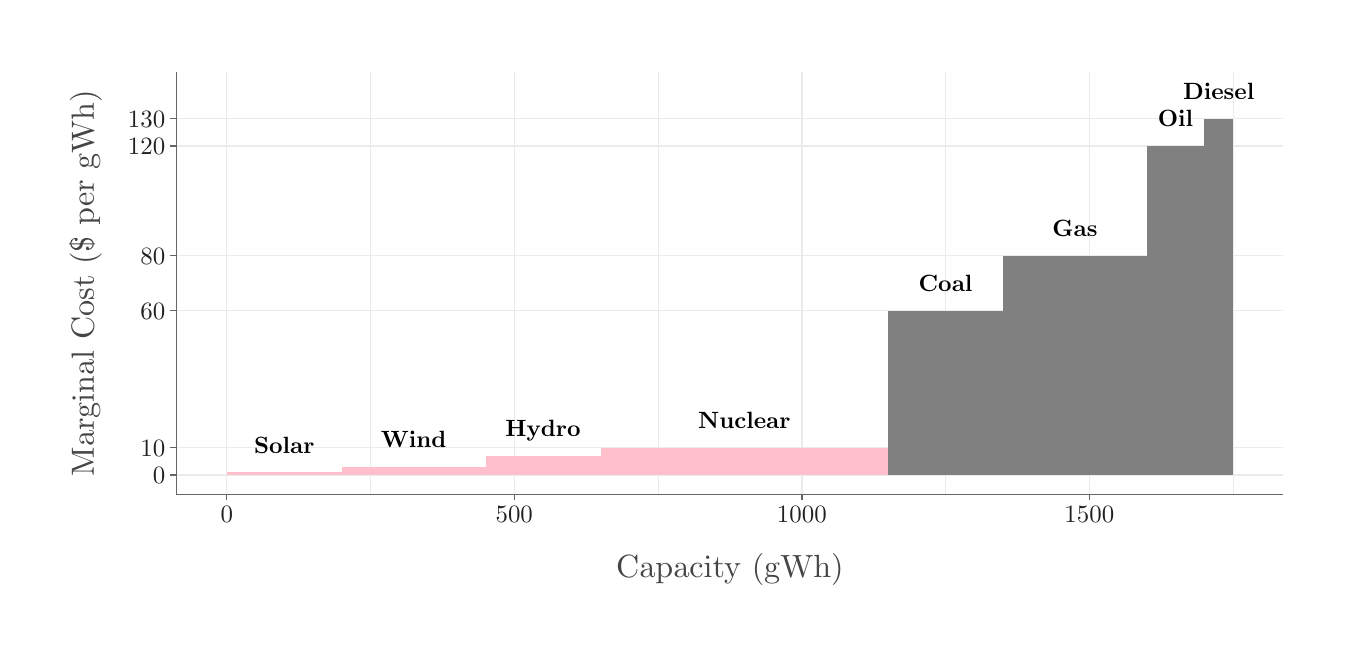
\begin{tikzpicture}[x=1pt,y=1pt]
\definecolor{fillColor}{RGB}{255,255,255}
\path[use as bounding box,fill=fillColor,fill opacity=0.00] (0,0) rectangle (469.75,216.81);
\begin{scope}
\path[clip] (  0.00,  0.00) rectangle (469.75,216.81);
\definecolor{fillColor}{RGB}{255,255,255}

\path[fill=fillColor] ( -0.00,  0.00) rectangle (469.76,216.81);
\end{scope}
\begin{scope}
\path[clip] ( 53.76, 48.21) rectangle (453.76,200.81);
\definecolor{fillColor}{RGB}{255,255,255}

\path[fill=fillColor] ( 53.76, 48.21) rectangle (453.75,200.81);
\definecolor{drawColor}{gray}{0.92}

\path[draw=drawColor,line width= 0.2pt,line join=round] (123.89, 48.21) --
	(123.89,200.81);

\path[draw=drawColor,line width= 0.2pt,line join=round] (227.78, 48.21) --
	(227.78,200.81);

\path[draw=drawColor,line width= 0.2pt,line join=round] (331.68, 48.21) --
	(331.68,200.81);

\path[draw=drawColor,line width= 0.2pt,line join=round] (435.57, 48.21) --
	(435.57,200.81);

\path[draw=drawColor,line width= 0.5pt,line join=round] ( 53.76, 55.14) --
	(453.76, 55.14);

\path[draw=drawColor,line width= 0.5pt,line join=round] ( 53.76, 65.05) --
	(453.76, 65.05);

\path[draw=drawColor,line width= 0.5pt,line join=round] ( 53.76,114.60) --
	(453.76,114.60);

\path[draw=drawColor,line width= 0.5pt,line join=round] ( 53.76,134.42) --
	(453.76,134.42);

\path[draw=drawColor,line width= 0.5pt,line join=round] ( 53.76,174.05) --
	(453.76,174.05);

\path[draw=drawColor,line width= 0.5pt,line join=round] ( 53.76,183.96) --
	(453.76,183.96);

\path[draw=drawColor,line width= 0.5pt,line join=round] ( 71.94, 48.21) --
	( 71.94,200.81);

\path[draw=drawColor,line width= 0.5pt,line join=round] (175.83, 48.21) --
	(175.83,200.81);

\path[draw=drawColor,line width= 0.5pt,line join=round] (279.73, 48.21) --
	(279.73,200.81);

\path[draw=drawColor,line width= 0.5pt,line join=round] (383.63, 48.21) --
	(383.63,200.81);
\definecolor{fillColor}{RGB}{255,192,203}

\path[fill=fillColor] ( 71.94, 55.14) rectangle (113.50, 56.13);

\path[fill=fillColor] (113.50, 55.14) rectangle (165.44, 58.12);

\path[fill=fillColor] (165.44, 55.14) rectangle (207.00, 62.08);

\path[fill=fillColor] (207.00, 55.14) rectangle (310.90, 65.05);
\definecolor{fillColor}{gray}{0.50}

\path[fill=fillColor] (310.90, 55.14) rectangle (352.46,114.60);

\path[fill=fillColor] (352.46, 55.14) rectangle (404.40,134.42);

\path[fill=fillColor] (404.40, 55.14) rectangle (425.18,174.05);

\path[fill=fillColor] (425.18, 55.14) rectangle (435.57,183.96);
\definecolor{drawColor}{RGB}{0,0,0}

\node[text=drawColor,anchor=base,inner sep=0pt, outer sep=0pt, scale=  0.85] at ( 92.72, 63.10) {\bfseries Solar};

\node[text=drawColor,anchor=base,inner sep=0pt, outer sep=0pt, scale=  0.85] at (139.47, 65.08) {\bfseries Wind};

\node[text=drawColor,anchor=base,inner sep=0pt, outer sep=0pt, scale=  0.85] at (186.22, 69.04) {\bfseries Hydro};

\node[text=drawColor,anchor=base,inner sep=0pt, outer sep=0pt, scale=  0.85] at (258.95, 72.02) {\bfseries Nuclear};

\node[text=drawColor,anchor=base,inner sep=0pt, outer sep=0pt, scale=  0.85] at (331.68,121.56) {\bfseries Coal};

\node[text=drawColor,anchor=base,inner sep=0pt, outer sep=0pt, scale=  0.85] at (378.43,141.38) {\bfseries Gas};

\node[text=drawColor,anchor=base,inner sep=0pt, outer sep=0pt, scale=  0.85] at (414.79,181.02) {\bfseries Oil};

\node[text=drawColor,anchor=base,inner sep=0pt, outer sep=0pt, scale=  0.85] at (430.38,190.93) {\bfseries Diesel};

\path[] ( 53.76, 48.21) rectangle (453.75,200.81);
\end{scope}
\begin{scope}
\path[clip] (  0.00,  0.00) rectangle (469.75,216.81);
\definecolor{drawColor}{gray}{0.40}

\path[draw=drawColor,line width= 0.5pt,line join=round] ( 53.76, 48.21) --
	( 53.76,200.81);
\end{scope}
\begin{scope}
\path[clip] (  0.00,  0.00) rectangle (469.75,216.81);
\definecolor{drawColor}{gray}{0.13}

\node[text=drawColor,anchor=base east,inner sep=0pt, outer sep=0pt, scale=  0.90] at ( 49.71, 52.04) {0};

\node[text=drawColor,anchor=base east,inner sep=0pt, outer sep=0pt, scale=  0.90] at ( 49.71, 61.95) {10};

\node[text=drawColor,anchor=base east,inner sep=0pt, outer sep=0pt, scale=  0.90] at ( 49.71,111.50) {60};

\node[text=drawColor,anchor=base east,inner sep=0pt, outer sep=0pt, scale=  0.90] at ( 49.71,131.32) {80};

\node[text=drawColor,anchor=base east,inner sep=0pt, outer sep=0pt, scale=  0.90] at ( 49.71,170.96) {120};

\node[text=drawColor,anchor=base east,inner sep=0pt, outer sep=0pt, scale=  0.90] at ( 49.71,180.86) {130};
\end{scope}
\begin{scope}
\path[clip] (  0.00,  0.00) rectangle (469.75,216.81);
\definecolor{drawColor}{gray}{0.40}

\path[draw=drawColor,line width= 0.5pt,line join=round] ( 51.51, 55.14) --
	( 53.76, 55.14);

\path[draw=drawColor,line width= 0.5pt,line join=round] ( 51.51, 65.05) --
	( 53.76, 65.05);

\path[draw=drawColor,line width= 0.5pt,line join=round] ( 51.51,114.60) --
	( 53.76,114.60);

\path[draw=drawColor,line width= 0.5pt,line join=round] ( 51.51,134.42) --
	( 53.76,134.42);

\path[draw=drawColor,line width= 0.5pt,line join=round] ( 51.51,174.05) --
	( 53.76,174.05);

\path[draw=drawColor,line width= 0.5pt,line join=round] ( 51.51,183.96) --
	( 53.76,183.96);
\end{scope}
\begin{scope}
\path[clip] (  0.00,  0.00) rectangle (469.75,216.81);
\definecolor{drawColor}{gray}{0.40}

\path[draw=drawColor,line width= 0.5pt,line join=round] ( 53.76, 48.21) --
	(453.76, 48.21);
\end{scope}
\begin{scope}
\path[clip] (  0.00,  0.00) rectangle (469.75,216.81);
\definecolor{drawColor}{gray}{0.40}

\path[draw=drawColor,line width= 0.5pt,line join=round] ( 71.94, 45.96) --
	( 71.94, 48.21);

\path[draw=drawColor,line width= 0.5pt,line join=round] (175.83, 45.96) --
	(175.83, 48.21);

\path[draw=drawColor,line width= 0.5pt,line join=round] (279.73, 45.96) --
	(279.73, 48.21);

\path[draw=drawColor,line width= 0.5pt,line join=round] (383.63, 45.96) --
	(383.63, 48.21);
\end{scope}
\begin{scope}
\path[clip] (  0.00,  0.00) rectangle (469.75,216.81);
\definecolor{drawColor}{gray}{0.13}

\node[text=drawColor,anchor=base,inner sep=0pt, outer sep=0pt, scale=  0.90] at ( 71.94, 37.96) {0};

\node[text=drawColor,anchor=base,inner sep=0pt, outer sep=0pt, scale=  0.90] at (175.83, 37.96) {500};

\node[text=drawColor,anchor=base,inner sep=0pt, outer sep=0pt, scale=  0.90] at (279.73, 37.96) {1000};

\node[text=drawColor,anchor=base,inner sep=0pt, outer sep=0pt, scale=  0.90] at (383.63, 37.96) {1500};
\end{scope}
\begin{scope}
\path[clip] (  0.00,  0.00) rectangle (469.75,216.81);
\definecolor{drawColor}{gray}{0.27}

\node[text=drawColor,anchor=base,inner sep=0pt, outer sep=0pt, scale=  1.16] at (253.76, 18.25) {Capacity (gWh)};
\end{scope}
\begin{scope}
\path[clip] (  0.00,  0.00) rectangle (469.75,216.81);
\definecolor{drawColor}{gray}{0.27}

\node[text=drawColor,rotate= 90.00,anchor=base,inner sep=0pt, outer sep=0pt, scale=  1.16] at ( 23.96,124.51) {Marginal Cost (\$ per gWh)};
\end{scope}
\end{tikzpicture}

  \end{figure}

  \item \points{20} Consider the merit-order curve in Figure \ref{fig:merit_order}.
  
  \begin{enumerate}  
    \item Why does the price of electricity vary throughout the day?
    
    \item If demand for electricity hits 1250 gWh, what will the market price be? 
    
    \item Using the concept of the `merit order effect', describe why increasing wind capacity could be so beneficial to consumers when demand is 1250 gWh.

    \item What is the Levalized Cost of Electricity and how does it differ from the Marginal Cost of producing a gWh? When considering construction of new energy sources, which is typically used by energy companies?
  \end{enumerate}

  \answer{
    \begin{enumerate}
      \item The price of electricity varies along the merit order curve since the amount of electricity demand varies over the day.
      
      \item The market price will be $\$60$ since the marginal cost of producing the $1250^{th}$ gWh is $\$60$.
      
      \item Adding wind capacity shifts the more expensive energy sources further out along the merit order curve. Whereas previously, coal had to be used for the $1250^{th}$ gWh of electricity, adding enough wind would allow nuclear to provide it, lowering the price of electricity to \$10 instead of \$60!
      
      \item The levalized cost of electricity is the \emph{average} cost of producing electricity when including the fixed cost of creating the energy generator. The marginal cost only includes the cost of operating it in that moment in time. 
      
      In general, the LCOE is used since it determines overall profitability of new construction.
    \end{enumerate}
  }
\end{enumerate}

\end{document}
